% Deal with strides ?


\documentclass[a4paper]{article}
\usepackage[latin9]{inputenc}

\usepackage{a4wide}
\usepackage{alltt,url}
\usepackage{todonotes,graphicx}

% Because we have examples with project headers with accents in UTF8,
% restranlate them in latin9...
\usepackage{listingsutf8}
\lstset{inputencoding=utf8/latin9,language=C,
  numbers=left, numberfirstline=false, stepnumber=5, basicstyle=\small,
  keywordstyle=\bf}

% For various symbols:
\let\OldRightarrow=\Rightarrow
\RequirePackage{marvosym}
\let\MarvosymRightarrow=\Rightarrow
\let\Rightarrow=\OldRightarrow
\RequirePackage{wasysym}
% Deal with conflicts between ifsym and marvosym by renaming conflicting
% symbols:
\let\MarvosymLightning=\Lightning
\let\Lightning=\UnTrucIndefini
\let\MarvosymLetter=\Letter
\let\Letter=\UnTrucIndefini
\let\MarvosymSun=\Sun
\let\Sun=\UnTrucIndefini
\RequirePackage[weather,misc,alpine,clock]{ifsym}
\usepackage{amssymb}

\begin{document}

\title{Some implementation details from the \texttt{smecc} compiler}

\author{Ronan~\textsc{Keryell}~(\url{Ronan.Keryell@silkan.com})}

\maketitle

\tableofcontents{}


\section{Introduction}
\label{sec:introduction}

\todo{The shorter the better.}

\section{OpenMP support}
\label{sec:openmp-support}

SME-C is a single program model (SPMD) based on OpenMP as its core model
with the OpenMP program being the controller of the whole application
driving some miscellaneous accelerators.

In our implementation, our compiler keep the OpenMP pragma in the output
main program.

The OpenMP pragma inside some piece of code mapped to accelerators may be
discarded if it does not make sense, for example if it is translated to an
OpenCL kernel or if it is replaced by a piece of hardware (FPGA...).


\section{Mapping on accelerators}
\label{sec:mapping-hardware}

The mapping of a function call on a specific piece of hardware can be
specified with pragma describing where the function is to be run and
optionally what arguments have to be transferred before execution and what
has to be retrieved after execution:
\begin{alltt}
#pragma smecy map(\emph{hardware[}, \emph{unit]*})
#pragma smecy arg(\emph{arg_id}, \emph{arg_clause[, arg_clause]...})
  some_function_call(...);
\end{alltt}

\begin{itemize}
\item \texttt{\emph{hardware}} is a symbol representing a hardware
  component of a given target such as \texttt{CPU}, \texttt{GPP},
  \texttt{GPU}, \texttt{PE}... They are target specific.
\item \texttt{\emph{unit}} entries are optional hierarchical instance
  number for a specific hardware part. This is typically an integer
  starting a 0. This hardware number can be an expression of the
  environment to be able to have a loop managing different accelerators.
\end{itemize}


\subsection{Mapping on OpenCL}
\label{sec:mapping-gpu}

The OpenCL can be used to target accelerators like GPU, STHORM or other
multicores.

For example the SME-C program

\lstinputlisting{examples/init_a.c}

is analyzed by the \texttt{smecc} compiler to generate an XML description
file to explain to the Par4All compiler that the \lstinline|init_array()|
function is parallel and has to be transformed to an OpenCL kernel, with
some memory transfers.

Then Par4All compiles the previous file to into 2 files, one for the host
program running on the main CPU:

\lstinputlisting{examples/init_a.p4a.c}

and an OpenCL file describing the kernel to be run on the accelerator:

\lstinputlisting{examples/p4a_wrapper_init_array.cl}

The OpenCL is indeed hidden in some higher-level macros beginning with
\verb|P4A_| to have terser code. For example
\verb|P4A_call_accel_kernel_2d| call the OpenCL API to compile the kernel,
stacking the call parameters and launching the kernel with the correct
NDRange. This allows to redirect more easily the compilation to CUDA for
example by changing the macro definitions.

Implementation limitations:
\begin{itemize}
\item an execution flow already mapped on a GPU kernel cannot launch
  another kernel because of the current OpenCL restriction\footnote{But
    this could be done in CUDA 5 with some recent K20 GPU.};
\item all the program has to be written in C, not C++.
\end{itemize}


\subsection{Mapping on STHORM MCA API}
\label{sec:prod-inform}

The STHORM platform is a MP-SoC with a 2-core ARM processor Cortex-A9
running Linux and an accelerator fabric with a 2D array of clusters, each
with 16 processing elements (PE).


\subsubsection{Addressing model}
\label{sec:addressing-model}

The MCA API contain the MCAPI message passing interface for embedded
system devices using an hierarchical addressing model made as a triplet
$<domain,node,port>$

\begin{figure}
  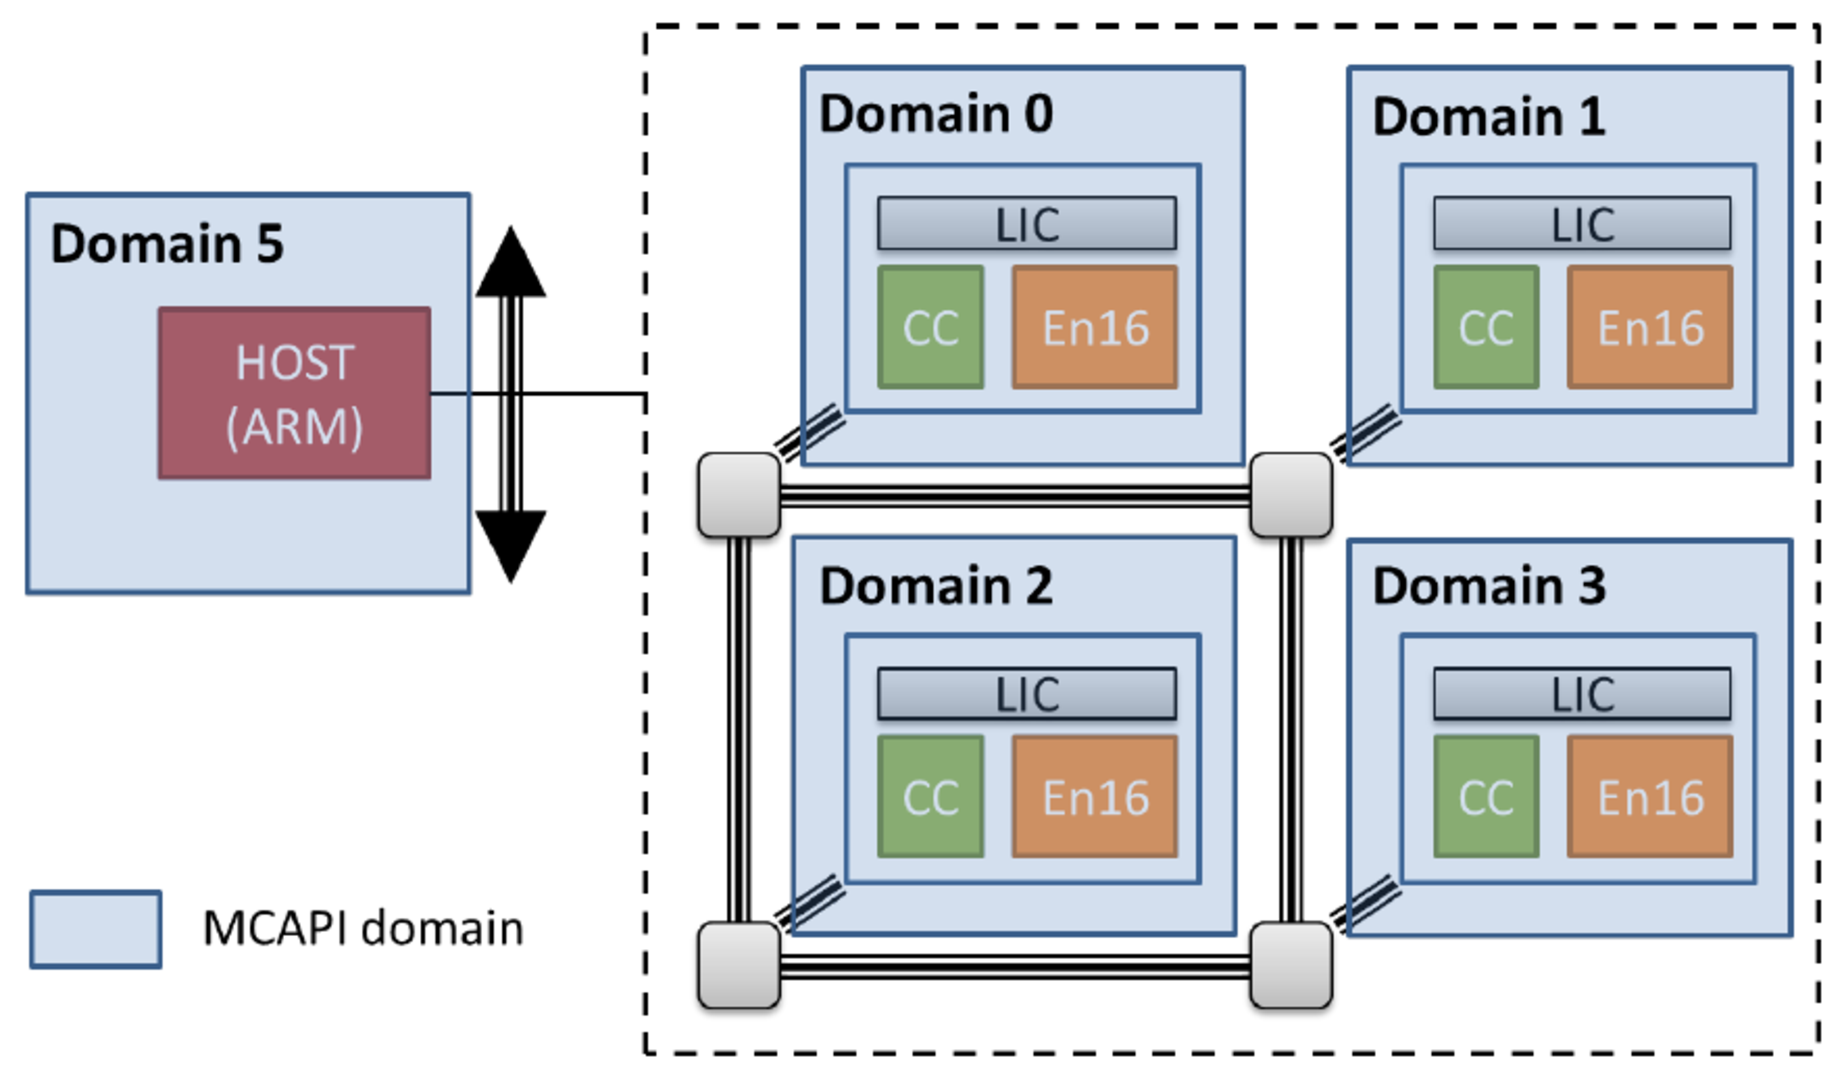
\includegraphics[width=\hsize]{figures/STHORM_MCAPI_mapping}
  \caption{MCAPI addressing model for a STHORM platform with $2\times2$
    clusters.}
  \label{fig:STHORM_MCAPI_mapping}
\end{figure}

The addressing model chosen by CEA for STHORM is to use the domain number
to select the clusters or the ARM host and use the node numbers to select
a PE inside the cluster selected by the domain number.

The domain numbering chosen by CEA for a cluster $(x,y)\in
(\mathbb{N}/n\mathbb{N})\times(\mathbb{N}/m\mathbb{N})$ inside a $n\times
m$ cluster machine is a plain 2D linearization:
\[
d = y \times n + x
\]
and the ARM host processor has the domain number $n\times m + 1$ with node
number 0.

An example for the $2\times2$ cluster simulator we use is shown on
Figure~\ref{fig:STHORM_MCAPI_mapping}.

Since the SME-C programming model is a SPMD model, by default all the code
runs on the host AMD processor, which is for example on domain 5 node 0,
perhaps with several OpenMP threads.

By using pragma such as
\begin{lstlisting}
#pragma smecy map(STHORM, 1, 3)
\end{lstlisting}
the execution of a function can be synchronously executed in the STHORM
fabric on the PE 3 of cluster 1.

Since for an execution on a PE the ARM processor has to launch a function
on it and there are many PEs, the function to be executed has to be large
grain.


\subsubsection{Memory model}
\label{sec:memory-model}

The memory model on STHORM is hierarchical and partially shared between
the ARM host processor and the fabric.

The global DDR memory, called the L3 memory, is shared in a weakly
coherent way by the host processor and the fabric PEs, through a global L2
cache.

This means that a multithread program running on the various cores and
with the right synchronization could run in parallel just by sharing
information though the L3 memory. Unfortunately, for power efficiency
reasons, there is no system like on a GPU to deal with coalescing multiple
accesses to the memory into a big one to improve
efficiency\todo{RK$\rightarrow$JM: does the L2 cache mitigates this?} of
the memory access. This means that the accesses will be slow.

To improve the efficiency, the local memory shared by the PEs of a cluster
or the private memory to a PE\todo{RK: double check it it makes sense.}
have to be used by placing the data in the right place.


\subsubsection{Runtime execution}
\label{sec:runtime-execution}

\todo{RK: express the following in some way with pragmas, comm}

Memory allocation

Our implementation is based on ST STHORM runtime. During nodes initialization and
channels connection we call ST memory allocators. User may want to use directly these memory
allocators. If it is the case user can refer to ST STHORM Runtime documentation [6]. Extract
of [6] which lists all the memory allocators accessible from CC :
\begin{lstlisting}
void * CC_l3Malloc (int size)
void CC_l3Free (void *ptr)
void * CC_enMalloc (int size)
void CC_enFree (void *ptr)
void * CC_malloc (int size)
void CC_free (void *ptr)
\end{lstlisting}


\subsubsection{Code transformation}
\label{sec:code-transformation}

The basic compilation scheme to generate MCAPI from the SME-C original
code is to generate several files:
\begin{itemize}
\item 1 host file running the host code on the Cortex-A9, an OpenMP C or
  C++ program with some calls to MCAPI functions to interact with the PEs;
\item as many source codes there are PEs, with the dual MCAPI function
  calls to get some data and to respond to the remote procedure calls from
  the hosts.
\end{itemize}

In this current implementation, since the host can chose at run-time the
PE on which a function will be executed, all the mapped functions are
loaded on the PEs and the real function to be executed is selected from a
previous MCAPI communication.

For example the \verb|examples/simple_map.c|
\begin{lstlisting}
#include <stdio.h>

#define N 10
#define M 5

void init(int* array, int size, int scale) {
  for (int i = 0; i < size; i++)
    array[i] = i*scale;
}

int main() {
  int tab[N][M];
  /* The schedule(static, 1) enforces each iteration to be executed in a
     different thread, whatever the number of CPU is: */
#pragma omp parallel for schedule(static, 1)
  for (int i = 0; i < N; i++) {
    // Map on STHORM cluster 0 PE i:
#pragma smecy map(STHORM, 0, i)        \
              arg(1,out,[N][M],/[i][]) \
              arg(2,in) \
              arg(3,in)
    init(&tab[i][0], M, i+1);
  }

  for (int i = 0; i < N; i++) {
    printf("Line %d :", i);
    for (int j = 0; j < M; j++)
      printf("%d ", tab[i][j]);
    puts("");
  }
  return 0;
}
\end{lstlisting}
is compiled to 2 files, a \verb|STHORM_rose_simple_map.c| file which is
to be compiled for the Cortex A9 ARM host with this content:
% This is the output examples/rose_simple_map.c after make in examples,
% without the definition of init()
\begin{lstlisting}
#include <stdio.h>
#define N 10
#define M 5
#include "smecy.h" 

int main()
{
  int tab[10UL][5UL];
/* The schedule(static, 1) enforces each iteration to be executed in a
     different thread, whatever the number of CPU is: */
  
#pragma omp parallel for schedule ( static, 1 )
  for (int i = 0; i < 10; i++) {
    SMECY_set(init,STHORM,0,i);
    SMECY_prepare_get_arg_vector(init,1,int,(tab[i] + 0),5,STHORM,0,i);
    SMECY_send_arg(init,2,int,5,STHORM,0,i);
    SMECY_send_arg(init,3,int,(i + 1),STHORM,0,i);
    SMECY_launch(init,3,STHORM,0,i);
    SMECY_get_arg_vector(init,1,int,(tab[i] + 0),5,STHORM,0,i);
  }
  for (int i = 0; i < 10; i++) {
    printf("Line %d :",i);
    for (int j = 0; j < 5; j++) 
      printf("%d ",tab[i][j]);
    puts("");
  }
  return 0;
}
\end{lstlisting}
the effect of \verb|SMECY_set(init,STHORM,0,i)| is to prepare the selection of
\texttt{init()} on the STHORM PE of coordinate $(0,i)$ by sending a first
MCAPI packet to prepare the execution of the following.



\todo{RK: rewrite the following by using a dispatch loop according to the
  SMECY\_set()
}
The \verb|STHORM_fabric.c| to be executed on the processors elements
of the STHORM fabric that will launch all the threads is constructed by
outlining the function calls to be executed to the fabric and only then
adding the MCAPI macros. This way, we can have a function object to be
given to the STHORM run-time that contains the MCAPI macros:
\begin{lstlisting}
#include "smecy.h"

// Provide extern call awaited by STHORM MCAPI implementation
void mcapi_domain_entry()
{

  SMECY_accelerator_loop_begin(init,STHORM,0,i);
  SMECY_set(init,STHORM,0,i);
  SMECY_prepare_get_arg_vector(init,1,int,(tab[i] + 0),5,STHORM,0,i);
  SMECY_send_arg(init,2,int,5,STHORM,0,i);
  SMECY_send_arg(init,3,int,(i + 1),STHORM,0,i);
  SMECY_launch(init,3,STHORM,0,i);
  SMECY_get_arg_vector(init,1,int,(tab[i] + 0),5,STHORM,0,i);
\end{lstlisting}
and for each MCAPI kernel to be launched on a PE, a file like
\verb|STHORM_PE_simple_map_init.c| with the code for the \verb|init|
function in this example with:
\begin{lstlisting}
#include <stdio.h>
#define N 10
#define M 5
#include "smecy.h"

void init(int *array,int size,int scale)
{
  for (int i = 0; i < size; i++)
    array[i] = (i * scale);
}

void STHORM_PE_simple_map_init()
{
  SMECY_accelerator_loop_begin(init,STHORM,0,i);
  SMECY_set(init,STHORM,0,i);
  SMECY_prepare_get_arg_vector(init,1,int,(tab[i] + 0),5,STHORM,0,i);
  SMECY_send_arg(init,2,int,5,STHORM,0,i);
  SMECY_send_arg(init,3,int,(i + 1),STHORM,0,i);
  SMECY_launch(init,3,STHORM,0,i);
  SMECY_get_arg_vector(init,1,int,(tab[i] + 0),5,STHORM,0,i);
  SMECY_accelerator_loop_end(init,STHORM,0,i);
}
\end{lstlisting}
All the \verb|SMECY_| have different meanings in the 3 different use
cases, so that mainly only one code is interpreted differently for the
right purpose.


\section{SMECY low level hardware API}
\label{sec:low-level-hardware}

To call real hardware accelerators, few C macros are needed to interface a
program running on some processor to a function running on another
processor or in some hardware accelerator.

Since the implementation may depend also on the processor calling the
macros (not the same IO bus will be used from an $x$86 or a DSP to call
the same operator), a global preprocessing symbol must be defined by the
compiler before using these macros, such as
\begin{lstlisting}
#define SMECY_LOCAL_PROC x86
\end{lstlisting}
or
\begin{lstlisting}
#define SMECY_LOCAL_PROC DSP
\end{lstlisting}

Few macros are necessary:
\todo{RK: to update with an automatic extraction}
\begin{lstlisting}
/* Prepare a processing element to execute a function

   @param pe is the symbol of a processing element, such as GPP, DSP, PE...
   @param[in] instance is the instance number of the processor element to use
   @param func is the function to load on the processor element

   pe is not a string because it is easy to make a string from it but not
   the opposite. The same for func
*/
#define SMECY_set(pe, instance, func) ...

/* Send a scalar argument to a function on a processing element

   @param pe is the symbol of a processing element, such as GPP, DSP, PE...
   @param[in] instance is the instance number of the processor element to use
   @param func is the function running on the processor element
   @param[in] arg is the argument instance to set
   @param type is the type of the scalar argument to send
   @param[in] val is the value of the argument to send
*/
#define SMECY_send_arg(pe, instance, func, arg, type, val) ...

/* Send a vector argument to a function on a processing element

   @param pe is the symbol of a processing element, such as GPP, DSP, PE...
   @param[in] instance is the instance number of the processor element to use
   @param func is the function to load on the processor element
   @param[in] arg is the argument instance to set
   @param type is the type of the vector element to send
   @param[in] addr is the starting address of the vector to read from
              caller memory
   @param[in] size is the length of the vector
*/
#define SMECY_send_arg_vector(pe, instance, func, arg, type, addr, size) ...

/* Launch the hardware function or remote program using previously loaded
   arguments

   @param pe is the symbol of a processing element, such as GPP, DSP, PE...
   @param[in] instance is the instance number of the processor element to use
   @param func is the function to load on the processor element

   A kernel can be launched several times without having to set/reset its function.
*/
#define SMECY_launch(pe, instance, func) ...

/* Get the return value of a function on a processing element

   @param pe is the symbol of a processing element, such as GPP, DSP, PE...
   @param[in] instance is the instance number of the processor element to use
   @param func is the function to load on the processor element
   @param type is the type of the scalar argument to send
   @return the value computed by the function
*/
#define SMECY_get_return(pe, instance, func, type) ...

/* Get a vector value computed by a function on a processing element

   @param pe is the symbol of a processing element, such as GPP, DSP, PE...
   @param[in] instance is the instance number of the processor element to use
   @param func is the function to load on the processor element
   @param[in] arg is the argument instance to retrieve
   @param type is the type of the vector element
   @param[out] addr is the starting address of the vector to write in
               caller memory
   @param[in] size is the length of the vector
*/
#define SMECY_get_arg_vector(pe, instance, func, arg, type, addr, size) ...

/* Prepare the retrieving of a vector value that will be computed by a
   function on a processing element.

   Typically, it can be used to allocate software or hardware resources
   for the later SMECY_get_arg_vector().

   @param pe is the symbol of a processing element, such as GPP, DSP, PE...
   @param[in] instance is the instance number of the processor element to use
   @param func is the function to load on the processor element
   @param[in] arg is the argument instance to retrieve
   @param type is the type of the vector element
   @param[out] addr is the starting address of the vector to write in
               caller memory
   @param[in] size is the length of the vector
*/
#define SMECY_future_get_arg_vector(pe, instance, func, arg, type, addr, size) ...

/* Reset a processing element to execute a function

   @param pe is the symbol of a processing element, such as GPP, DSP, PE...
   @param[in] instance is the instance number of the processor element to use
   @param func is the function to unload from the processor element

   This is used for example to remove consuming resources to decrease
   power. Giving here the function name may be useful for weird case to
   avoid having short-circuit between CLB in a FPGA during unconfiguring stuff
*/
#define SMECY_reset(pe, instance, func) ...
\end{lstlisting}
There is also a macro for an asynchronous call and to wait for completion.


\section{Compilation}
\label{sec:compilation}

\subsection{Example of OpenCL mapping}
\label{sec:example-opencl-mapp}

A typical mapping of the SMECY low level hardware API shown on
\S~\ref{sec:low-level-hardware} would be organized as follows:
\begin{itemize}
\item \verb|SMECY_set(PE, proc & 7, invert_vector)|:\\
  \texttt{clCreateProgramFromSource()} +
  \texttt{clBuildProgramExecutable()} + \texttt{clCreateKernel()}
\item \verb|SMECY_send_arg(PE, proc & 7, invert_vector, 1, int, LINE_SIZE)|:\\
  \texttt{clSetKernelArg()}
\item \verb|SMECY_send_arg_vector(PE, proc & 7, invert_vector, 2, int,...)|:\\
  \texttt{clCreateBuffer()} + \texttt{clSetKernelArg()} (+
  \texttt{clEnqueueWriteBuffer()})
\item \verb|SMECY_launch(PE, 0, invert_vector)|:\\
  \texttt{clExecuteKernel()}
\item \verb|SMECY_get_arg_vector(PE, proc & 7, invert_vector, 3, ...)|:\\
  \texttt{clEnqueueReadBuffer()}
\end{itemize}


\subsection{Example of EdkDSP mapping}
\label{sec:example-edkdsp-mapp}


\subsection{OpenMP support}
\label{sec:openmp-support-1}

From the programmer point of view it may be equivalent to have
\begin{itemize}
\item an OpenMP compiler generating SMECY API code such as the parallelism
  between SMECY target accelerators is run by OpenMP threads dealing each
  one with an hardware resource sequentially in a synchronous way;
\item or a SMECY compiler understanding the OpenMP syntax and generating
  directly some parallel execution of SMECY accelerators in an
  asynchronous way.
\end{itemize}


\subsection{Doxygen qualifier}
\label{sec:doxygen-qualifier}

In the Doxygen documentation mark-up language used in comments to detail
various entities of a program, there are information such as \texttt{in},
\texttt{out} or \texttt{inout} qualifier on function parameters that can
be used to generate the right communication with some hardware
accelerators.


\subsection{C qualifier}
\label{sec:c-qualifier}

Qualifiers such as \texttt{const} attribute qualifier, address space
names, register names, accumulator, saturation, etc. are used to generate
the right target function or instruction.


\subsection{Generating communications from pragma}
\label{sec:pragma}

Of course the pragma information is heavily used in the compilation
process.

For example to generate correct communication, the mapping information is
used, and from the used/defined information plus optional remapping
information, a real communication with an API is used.

\begin{lstlisting}
void
invert_vector(int line_size,
          int input_line[line_size],
          int output_line[line_size]) {
  for(int i = 0; i < line_size; i++)
    output_line[i] = 500 - input_line[i];
}
  [...]
  int image[HEIGHT][WIDTH];
  [...]
#pragma smecy map(PE, proc & 7)         \
              arg(2, in, [1][LINE_SIZE])    \
              arg(3, out, [1][LINE_SIZE])
    // Invert an horizontal line:
    invert_vector(LINE_SIZE,
          &image[HEIGHT - 20 - proc][WIDTH/2 + 2*proc],
          &image[HEIGHT - 20 - proc][WIDTH/2 + 2*proc]);
\end{lstlisting}
can be compiled into
\begin{lstlisting}
  int image[HEIGHT][WIDTH];
  /* First prepare the PE #(proc & 7) hardware to execute invert_vector.
     That may be used to load some program or microcode, reconfigure a
     FPGA, load/compile an OpenCL kernel... */
  SMECY_set(PE, proc & 7, invert_vector);
  /* Send the WIDTH integer as arg 1 on invert_vector hardware function on
     PE #(proc & 7): */
  SMECY_send_arg(PE, proc & 7, invert_vector, 1, int, LINE_SIZE);
  /* Send a vector of int of size LINE_SIZE as arg 2 on invert_vector
     hardware function on PE #(proc & 7): */
  SMECY_send_arg_vector(PE, proc & 7, invert_vector, 2, int,
                        &image[HEIGHT - 20 - proc][WIDTH/2 + 2*proc], LINE_SIZE);
  // Launch the hardware function or remote program:
  SMECY_launch(PE, 0, invert_vector);
  /* Get a vector of int of size LINE_SIZE as arg 3 on invert_vector
     hardware function on PE #(proc & 7): */
  SMECY_get_arg_vector(PE, proc & 7, invert_vector, 3, &image[HEIGHT - 20 - proc]
                                                             [WIDTH/2 + 2*proc],
                       LINE_SIZE);
\end{lstlisting}
with low level macros described in \S~\ref{sec:low-level-hardware}.

\lstinline|invert_vector()| is either an already implemented function in a
hardware library, or it is compiled by a target specific compiler with
some callable interface.

For more complex calls needing remapping, such as:
\begin{lstlisting}
    int input_line[LINE_SIZE];
    int output_line[LINE_SIZE];
    /* We need to remap data in the good shape. The compiler should use
       the remapping information to generate DMA transfer for example and
       remove input_line array */
    SMECY_remap_int2D_to_int1D(HEIGHT, WIDTH, HEIGHT/3, 30 + 20*proc,
                   LINE_SIZE, 1, image,
                   LINE_SIZE, input_line);
    // Each iteration is on a different PE in parallel:
#pragma smecy map(PE, proc) arg(2, in, [LINE_SIZE]) arg(3, out, [LINE_SIZE])
    invert_vector(LINE_SIZE, input_line, output_line);
    SMECY_remap_int1D_to_int2D(LINE_SIZE, output_line,
                   HEIGHT, WIDTH, HEIGHT/3, 30 + 20*proc,
                   LINE_SIZE, 1, image);
\end{lstlisting}
is compiled by using other hardware interfaces involving more complex DMA:
\begin{lstlisting}
  // May not be useful if this function is already set:
  SMECY_set(PE, proc & 7, invert_vector);
  /* Send the WIDTH integer as arg 1 on invert_vector hardware function on
     PE #(proc & 7): */
  SMECY_send_arg(PE, proc & 7, invert_vector, 1, int, LINE_SIZE);
  /* Send a vector of int of size LINE_SIZE as arg 2 on invert_vector
     hardware function on PE #(proc & 7) but read as a part of a 2D array: */
  smecy_send_arg_int_DMA_2D_PE_0_invert_vector(3, &image[HEIGHT - 20 - proc]
                                                        [WIDTH/2 + 2*proc],
                                               HEIGHT, WIDTH, HEIGHT/3, 30 + 20*proc,
                                               LINE_SIZE, 1);
  SMECY_send_arg_DMA_2D_to_1D(PE, proc & 7, invert_vector, 2, int,
                              &image[HEIGHT - 20 - proc][WIDTH/2 + 2*proc],
                              HEIGHT, WIDTH, HEIGHT/3, 30 + 20*proc,
                              LINE_SIZE, 1);
  // Launch the hardware function or remote program:
  SMECY_launch(PE, 0, invert_vector);
  SMECY_get_arg_DMA_1D_to_2D(PE, proc & 7, invert_vector, 3, int,
                             &image[HEIGHT - 20 - proc][WIDTH/2 + 2*proc],
                             HEIGHT, WIDTH, HEIGHT/3, 30 + 20*proc,
                             LINE_SIZE, 1);
\end{lstlisting}


\subsection{Compilation for streaming computing}
\label{sec:comp-stre-comp}

\todo{RK: not longer implemented this way}
If we come back on the example shown in \S~\ref{sec:pipelined-example} on
page~\pageref{sec:pipelined-example}, this program is given to the
source-to-source stream compiler that may generate the following output
(only partially shown, the type definitions are missing):
\begin{lstlisting}
/* Definition of procedures */
int main(void)
{
    typ_7 data_buffer;
    typ_21 data12Link;
    data12Link = pth_CreateDbLink(512);
    pth_CreateProcess((&__Node1), data12Link);
    pth_CreateProcess((&__Node2), data12Link);
    pause();
    return 0;
}

static void __outlinedproc2(typ_9 data_buffer)
{
    Consume(((typ_4)data_buffer));
}

static void __outlinedproc1(typ_9 data_buffer)
{
    Produce(((typ_4)data_buffer));
}

static void __Node1(typ_21 data12Link)
{
    typ_9 data_bufferOut;
    typ_4 tmp0;
    typ_4 tmp1;
    tmp0 = DbLinkGetInitBuff(data12Link);
    data_bufferOut = ((typ_9)tmp0);
    while(1){
        __outlinedproc1(data_bufferOut);
        tmp1 = DbLinkPutData(data12Link);
        data_bufferOut = ((typ_9)tmp1);
    }
}

static void __Node2(typ_21 data12Link)
{
    typ_9 data_bufferIn;
    typ_4 tmp0;
    while(1){
        tmp0 = DbLinkGetData(data12Link);
        data_bufferIn = ((typ_9)tmp0);
        __outlinedproc2(data_bufferIn);
    }
}
\end{lstlisting}
The last two functions are \verb|__Node1()| and \verb|__Node2()|. These
are the functions that run in the two processes. These two functions are
the wrappers around the user code, which is embedded in the two
\verb|__oulined...| functions. These wrappers take care of the
data communications. For every communication channel, they manage a
double-buffered scheme that minimizes the amount of copying.

In more realistic settings than this simple send/receive scheme,
the wrapper function become quickly more complex and non-trivial
to maintain manually.

The generated code contains calls to the following communication
library:
\begin{lstlisting}
/*
 * Create a double buffered communication link,
 * with each buffer the given size in bytes */
DbLink createDbLink( int size ) ;
/*
 * Get a pointer to a free output buffer from the
 * link. The pointer must be given back in the
 * call to DbLinkPutData */
void *DbLinkGetInitBuf( DbLink outputLink ) ;
/*
 * Get a pointer to data out of the link. This
 * is a read action of the link. The data pointed
 * to is valid until the next read. */
void *DbLinkGetData( DbLink inputLink ) ;
/*
 * Output the data pointed to over the link. The
 * pointer must have been previously obtained from
 * the link. */
data_bufferOut = DbLinkPutData( data_bufferOut ) ;
\end{lstlisting}

And finally there is also the process creation call:
\begin{lstlisting}
int pth_CreateProcess( int (*f)(), ... );
\end{lstlisting}
This library is not intended to become part of the SMECY-API described for
example in \S~\ref{sec:smecy-api} or \ref{sec:low-level-hardware}.
Instead, the library is intended for easy porting to SMECY-API, while
taking advantage of the most efficient communication implementation for
the specific target architecture. Currently, a \texttt{pthread}s-based
implementation exists.

This is just an example of a compilation path and it should be easy to
generate a C++ TBB (Thread Building Block) target code using for example
the \verb|tbb::pipeline|, a more low-level OpenMP runtime based on
\texttt{parallel sections} or \texttt{parallel task} pragma, or even an
MPI or MCA API for distributed memory execution.


\subsection{Geometric inference}
\label{sec:geometric-inference}

In the OpenMP SMP model, there is a global memory (well, with a weak
coherence model) that may not exist in the execution model of a given
target. For example, even if 2 hardware accelerators exchange information
through memory according to the high-level programming model, in the real
world we may have 2 processors communicating through message passing with
MCAPI on a NoC or 2 hardware accelerators connected through a pipeline.

To solve this issue, we use the OpenMP global memory like a scoreboard
memory that is used to symbolically relate all the data flows and
generates various communication schemes.

Since the memory dependencies are expresses by hyperparallelepipedes, we
can do some intersection analysis to compute if a communication is needed
or not between 2 devices of the target.



\end{document}


%%% Local Variables:
%%% mode: latex
%%% ispell-local-dictionary: "american"
%%% TeX-auto-untabify: t
%%% TeX-PDF-mode: t
%%% End:

% vim:spell spelllang=en
